\documentclass[tikz]{standalone}

\definecolor{morange}{RGB}{255,127,14}
\definecolor{mblue}{RGB}{31,119,180}
\definecolor{mred}{RGB}{214,39,40}
\definecolor{mpurple}{RGB}{148,103,189}
\definecolor{mgreen}{RGB}{44,160,44}

\newcommand*{\colIn}{morange}%
\newcommand*{\colEnc}{mpurple}%
\newcommand*{\colIntr}{mred}%
\newcommand*{\colDec}{mpurple}%
\newcommand*{\colOut}{mgreen}%
\newcommand*{\colSym}{mblue}%

\newcommand*{\arrowLength}{1}%

\newcommand*{\xMin}{1}%
\newcommand*{\xMax}{8}%
\newcommand*{\xMaxEnc}{4}%
\newcommand*{\xMaxIntr}{2}%
\newcommand*{\xMaxDec}{4}%

\newcommand*{\xin}{0}%
\newcommand*{\xinsym}{\xin+\arrowLength+2}%
\newcommand*{\xenc}{\xinsym+\arrowLength+2}%
\newcommand*{\xencsym}{\xenc+\arrowLength+2}%
\newcommand*{\xintr}{\xencsym+\arrowLength+2}%
\newcommand*{\xdecsym}{\xintr+\arrowLength+2}%
\newcommand*{\xdec}{\xdecsym+\arrowLength+2}%
\newcommand*{\xoutsym}{\xdec+\arrowLength+2}%
\newcommand*{\xout}{\xoutsym+\arrowLength+2}%


\begin{document}
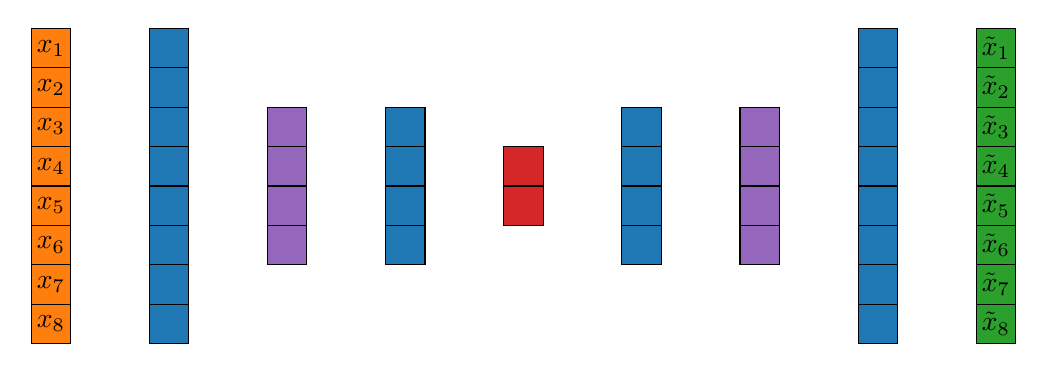
\begin{tikzpicture}[scale=0.5]

    \begin{scope}
        \foreach \i in {\xMin,...,\xMax} {
            \draw [rectangle, draw, fill=\colIn] (\xin,\xMax/2-\i) rectangle (\xin+1,\xMax/2-\i+1) node [pos=.5] {$x_\i$};
        }
    \end{scope}

    \path [draw,->, white] (\xin+1.5,0) -- (\xinsym-0.5,0) node [pos=0.5,above,align=left] {\color{white}$\psi_1$};

    \begin{scope}
        \foreach \i in {\xMin,...,\xMax} {
            \draw [rectangle, draw, fill=\colSym] (\xinsym,\xMax/2-\i) rectangle (\xinsym+1,\xMax/2-\i+1) node [pos=.5] {};
        }
    \end{scope}

    \path [draw,->, white] (\xinsym+1.5,0) -- (\xenc-0.5,0) node [pos=0.5,above,align=left] {\color{white}$A_1^+$};

    \begin{scope}
        \foreach \i in {\xMin,...,\xMaxEnc} {
            \draw [rectangle, draw, fill=\colEnc] (\xenc,\xMaxEnc/2-\i) rectangle (\xenc+1,\xMaxEnc/2-\i+1) node {};
        }
    \end{scope}

    \path [draw,->, white] (\xenc+1.5,0) -- (\xencsym-0.5,0) node [pos=0.5,above,align=left] {\color{white}$\psi_2$};

    \begin{scope}
        \foreach \i in {\xMin,...,\xMaxEnc} {
            \draw [rectangle, draw, fill=\colSym] (\xencsym,\xMaxEnc/2-\i) rectangle (\xencsym+1,\xMaxEnc/2-\i+1) node {};
        }
    \end{scope}

    \path [draw,->, white] (\xencsym+1.5,0) -- (\xintr-0.5,0) node [pos=0.5,above,align=left] {\color{white}$A_2^+$};

    \begin{scope}
        \foreach \i in {\xMin,...,\xMaxIntr} {
            \draw [rectangle, draw, fill=\colIntr] (\xintr,\xMaxIntr/2-\i) rectangle (\xintr+1,\xMaxIntr/2-\i+1) node {};
        }
    \end{scope}

    \path [draw,->, white] (\xintr+1.5,0) -- (\xdecsym-0.5,0) node [pos=0.5,above,align=left] {\color{white}$A_3$};

    \begin{scope}
        \foreach \i in {\xMin,...,\xMaxEnc} {
            \draw [rectangle, draw, fill=\colSym] (\xdecsym,\xMaxEnc/2-\i) rectangle (\xdecsym+1,\xMaxEnc/2-\i+1) node {};
        }
    \end{scope}

    \path [draw,->, white] (\xdecsym+1.5,0) -- (\xdec-0.5,0) node [pos=0.5,above,align=left] {\color{white}$\psi_3$};

    \begin{scope}
        \foreach \i in {\xMin,...,\xMaxDec} {
            \draw [rectangle, draw, fill=\colDec] (\xdec,\xMaxDec/2-\i) rectangle (\xdec+1,\xMaxDec/2-\i+1) node {};
        }
    \end{scope}

    \path [draw,->, white] (\xdec+1.5,0) -- (\xoutsym-0.5,0) node [pos=0.5,above,align=left] {\color{white}$A_4$};

    \begin{scope}
        \foreach \i in {\xMin,...,\xMax} {
            \draw [rectangle, draw, fill=\colSym] (\xoutsym,\xMax/2-\i) rectangle (\xoutsym+1,\xMax/2-\i+1) node [pos=.5] {};
        }
    \end{scope}

    \path [draw,->, white] (\xoutsym+1.5,0) -- (\xout-0.5,0) node [pos=0.5,above,align=left] {\color{white}$\psi_4$};

    \begin{scope}
        \foreach \i in {\xMin,...,\xMax} {
            \draw [rectangle, draw, fill=\colOut] (\xout,\xMax/2-\i) rectangle (\xout+1,\xMax/2-\i+1) node [pos=.5] {$\tilde{x}_\i$};
        }
    \end{scope}


%   \node[rectangle,draw,fill=teal!,text width=.3cm] (11) at (0,0) {$x_1$ \\ $x_2$ \\ $x_3$ \\ $x_4$ \\ $x_5$ \\ $x_6$ \\ $x_7$ \\ $x_8$};
%   \node[rectangle,draw,fill=teal!,text width=.3cm] (12) at (1,0) {$x_1$ \\ $x_2$ \\ $x_3$ \\ $x_4$ \\ $x_5$ \\ $x_6$ \\ $x_7$ \\ $x_8$};
%   \node[rectangle,draw,fill=olive!,text width=.3cm] (21) at (2,0) {$x_1$ \\ $x_2$ \\ $x_3$ \\ $x_4$ };
%   \node[rectangle,draw,fill=olive!,text width=.3cm] (22) at (3,0) {$x_1$ \\ $x_2$ \\ $x_3$ \\ $x_4$ };
%   \node[rectangle,draw,fill=lightgray!,text width=.3cm] (3) at (4,0) {$x_1$ \\ $x_2$ };
%   \node[rectangle,draw,fill=olive!,text width=.3cm] (41) at (5,0) {$x_1$ \\ $x_2$ \\ $x_3$ \\ $x_4$ };
%   \node[rectangle,draw,fill=olive!,text width=.3cm] (42) at (6,0) {$x_1$ \\ $x_2$ \\ $x_3$ \\ $x_4$ };
%   \node[rectangle,draw,fill=teal!,text width=.3cm] (51) at (7,0) {$x_1$ \\ $x_2$ \\ $x_3$ \\ $x_4$ \\ $x_5$ \\ $x_6$ \\ $x_7$ \\ $x_8$};
%   \node[rectangle,draw,fill=teal!,text width=.3cm] (52) at (8,0) {$x_1$ \\ $x_2$ \\ $x_3$ \\ $x_4$ \\ $x_5$ \\ $x_6$ \\ $x_7$ \\ $x_8$};
%   \path[draw,->] (11.east) -- (12.west) node[pos=0.5,above,align=left] {$\psi_1$};
%   \path[draw,->] (21.east) -- (22.west) node[pos=0.5,above,align=left] {$\psi_2$};
%   \path[draw,->] (41.east) -- (42.west) node[pos=0.5,above,align=left] {$\psi_3$};
%   \path[draw,->] (51.east) -- (52.west) node[pos=0.5,above,align=left] {$\psi_4$};
%   \path[draw,->] (12.east) -- (21.west) node[pos=0.5,above,align=left] {$A_1$};
%   \path[draw,->] (22.east) -- (3.west) node[pos=0.5,above,align=left] {$A_2$};
%   \path[draw,->] (3.east) -- (41.west) node[pos=0.5,above,align=left] {$A_3^+$};
%   \path[draw,->] (42.east) -- (51.west) node[pos=0.5,above,align=left] {$A_4^+$};

\end{tikzpicture}
\end{document}
